
\section{Results}
The Stack of Tasks (SoT) controller has also been deployed and tested for achieving different postures on the setup in Fig. \ref{fig:TUDSetup}. We are actively working on extending the behavior to path following and eventually integrate in accordance with the reactive collision avoidance architecture shown in Fig. \ref{fig:dca}. 


\subsection{Integrated evaluation}
\hypersetup{colorlinks, linkcolor=blue}
The integration of all the components described earlier has been evaluated on a simulation of the orange sorting setup as shown in Fig. \ref{fig:TOMMSimulation}.

\begin{figure}[h]
\centering
\resizebox{1.0\columnwidth}{!}{\includegraphics{doa/images/tomm_simulation.png}}\\[-10pt]
\caption[]{Orange sorting scenario in simulation.The red point cloud is a simulated obstacle.}
\label{fig:TOMMSimulation}
\end{figure}
The evaluation is done in a ROS based gazebo environment with the skin sensors simulated using the flexible collision library to project the distance between objects to sensor range measurements. 
These measurements are mapped to signals compatible in dynamic graph framework using a bridge component to allow its use in the SoT controller. The collision avoidance component computes the point 
distance and jacobian of each and every skin cell configured  essential to feed as an inequality constraint to the solver which backs the SoT controller. The planning component having the capability 
to plan with point cloud data has a Moveit python interface to query motion plan requests. The response is a set of way points which is then linearly interpolated to instantaneous joint position commands
to a path tracking task in the SoT. The SoT controller also has a python interface which makes it easy to design application scenarios.

The combined use of a reactive motion planner and a hierarchical reactive SoT controller with skin data makes it a good candidate for applying dynamical obstacle avoidance in factory environments.
A video result of the same is available \href{https://youtu.be/uLStjR7mpOI}{here}.

% \section{Experimental Illustration}
% We experimented a scenario to verify reactive trajectory execution to achieve a pre-grasp end effector configuration. The SOT framework is embedded in a ROS based real time controller running on a PR2, a mobile manipulation platform. The mobile base and the arms in this platform makes it apt for our scenarios which validates the practical advantage of the proposed methodology. A skin sensor is mounted on the forearm of the left arm . This scenario focuses on executing a simple trajectory on the left arm from an initial position (in the figure \ref{fig:init}) to reach a pregrasp position(in the figure \ref{fig:traj4}). The desired trajectory doesn't involve any movement in joints other than the left arm but they are not constrained to move as a part of the set-up. This figure \ref{ExperimentA} shows the tasks in the stack with priorities decreasing from top to bottom. 
%  The SOT controller executes a preplanned trajectory which is fed to the joint trajectory execution task in the stack. The respective end-effector pose of the trajectory at each instant is fed to an end effector pose task with a priority higher than the joint trajectory task.
%     \begin{figure}[h]
%       \centering
%       \includegraphics[scale=0.21]{doa/images/expillustration.png}
%       \caption{Robot Architecture of the Illustration Scenario}
%       \label{ExperimentA}
%    \end{figure}
 
% The planned way points are fed to a trajectory
% interpolator component which computes instantaneous joint position control
% signals to execute a joint posture task. The skin sensor component being a
% ROS based node publishes topics which are converted to signals in Dynamic
% Graph to be used by collision avoidance component necessary to compute
% information for feeding an inequality task in the solver stack. This is how
% safety and trajectory tracking are executed simultaneously. The adaptability of the controller without compromising the end goal comes
% from the pose task inserted between these tasks. The trajectory interpolator also sends a forward kinematic signal of the end effector corresponding to the joint trajectory point every instant. This allows the controller to stick with the
% plan as close as possible without violating the safety constraints and
% compromising the end goal of the scenario.



% \begin{figure}[!htb]
% \minipage{0.25\textwidth}
%   \includegraphics[width=\linewidth]{doa/images/traj1.png}
%   \caption{Initial Posture}\label{fig:init}
% \endminipage
% \minipage{0.25\textwidth}
%   \vspace{0.15\textwidth}
%   \includegraphics[width=\linewidth]{doa/images/traj4.png}
%   \caption{The robot while executing the trajectory with an actor's hand in proximity.}\label{fig:traj2}
% \endminipage\hfill
% \minipage{0.25\textwidth}%
%   \vspace{0.2\textwidth}
%   \includegraphics[width=\linewidth]{doa/images/traj8.png}
%   \caption{Base motion to avoid proximity with hand simulated yet the wrist pose is maintained.}\label{fig:traj3}
% \endminipage
% \minipage{0.25\textwidth}%
% \vspace{0.13\textwidth}
%   \includegraphics[width=\linewidth]{doa/images/traj11.png}
%   \caption{Final Posture after the sensor error is within the safe region.}\label{fig:traj4}
% \endminipage
% \end{figure}
   
%     \begin{figure}[!h]
%       \centering
%       \includegraphics[scale=0.35]{doa/images/BasePlot-eps-converted-to-crop.pdf}
%       \caption{Base Motion Trajectory Evolution}
%       \label{figurebase}
%    \end{figure}  
   
%   The experiment is done in simulation and the skin sensor error is varied using a software handle. The pink colored vector on the left forearm seen in the figures \ref{fig:init} -\ref{fig:traj4} correspond to unit normal distance vector determining the direction of the robot motion in the workspace to avoid collision. The figure \ref{figurebase} shows the evolution of the base position when the sensor error oscillates between safe and unsafe regions of proximity with an obstacle. They clearly shows the base motion deviating from the reference trajectory but gets back its desired state when the error is in the safe region. The important thing is the pose of the wrist is unchanged except the yaw ( which was relaxed in the pose task to afford base motion to avoid collision while it maintains the pose)
%    \begin{figure}[!h]
%       \centering
%       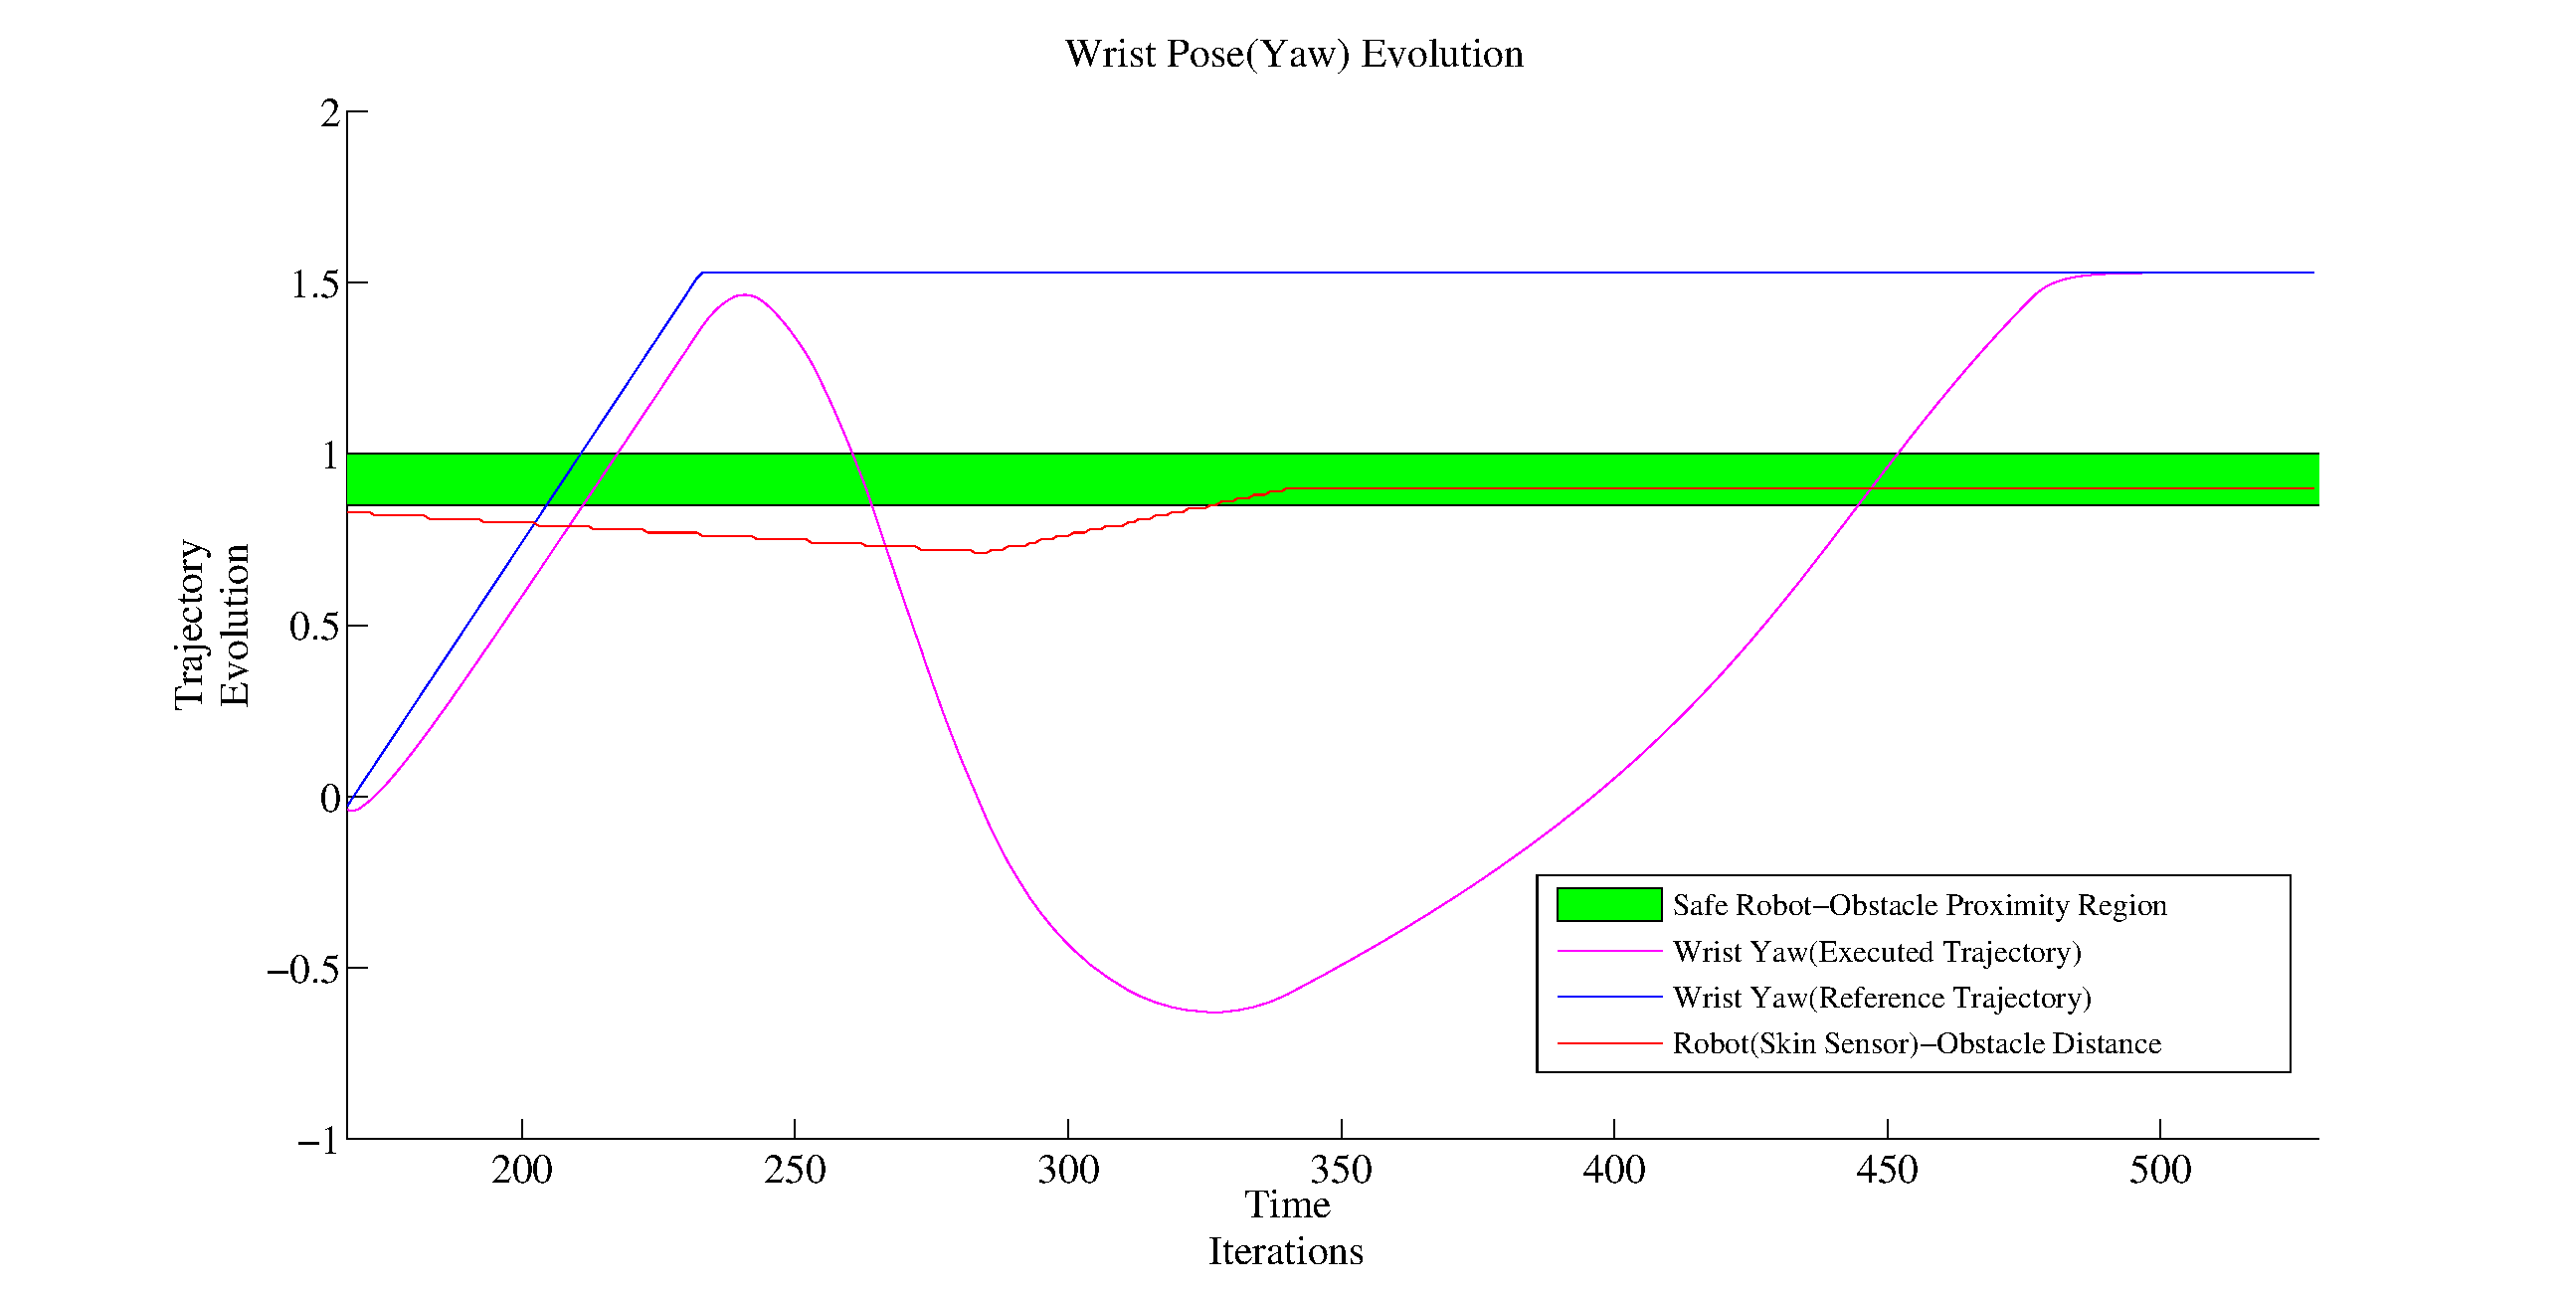
\includegraphics[scale=0.2]{doa/images/WristYawTrajectoryEvolution.eps}
%       \caption{Wrist Pose (Yaw) Evolution}
%       \label{poseYaw}
%    \end{figure}
  
% The figure \ref{poseYaw} shows the evolution of the wrist pose(yaw) of the robot which shows the connection with the base motion to compensate for the collision avoidance but yet the wrist roll and pitch in workspace doesn't change. The simple scenario could be extended to complex scenarios by figuring out the appropriate tasks corresponding to the scenario. The future work will be focused on a generic methodology to generate tasks in the stack just by specifying the scenario and feeding a trajectory.
